\documentclass{wissdoc}
% Autor: Roland Bless 1996-2009, bless <at> kit.edu
% ----------------------------------------------------------------
% Diplomarbeit - Hauptdokument
% ----------------------------------------------------------------
%%
%% $Id: thesis.tex 65 2012-05-10 10:32:11Z bless $
%%
%
% Zum Erstellen zweiseitiger PDFs (für Buchdruck) in der Datei "wissdoc.cls" folgende Zeile abändern:
%
% \LoadClass[a4paper,12pt,oneside]{book} % diese Klasse basiert auf ``book''
% in
%\LoadClass[a4paper,12pt,titlepage]{book} % diese Klasse basiert auf ``book''
%
%
% wissdoc Optionen: draft, relaxed, pdf --> siehe wissdoc.cls
% ------------------------------------------------------------------
% Weitere packages: (Dokumentation dazu durch "latex <package>.dtx")
\usepackage[numbers,sort&compress]{natbib}
\usepackage{hyperref}
\usepackage{csquotes}
\usepackage[english]{babel}

% \usepackage{varioref}
% \usepackage{verbatim}
% \usepackage{float}    %z.B. \floatstyle{ruled}\restylefloat{figure}
% \usepackage{subfigure}
% \usepackage{fancybox} % für schattierte,ovale Boxen etc.
% \usepackage{tabularx} % automatische Spaltenbreite
% \usepackage{supertab} % mehrseitige Tabellen
% \usepackage[svnon,svnfoot]{svnver} % SVN Versionsinformation 
%% ---------------- end of usepackages -------------

%\svnversion{$Id: thesis.tex 65 2012-05-10 10:32:11Z bless $} % In case that you want to include version information in the footer

%% Informationen für die PDF-Datei
\hypersetup{
 pdfauthor={Sven Fiergolla},
 pdftitle={Improvements on RLE by preprocessing}
 pdfsubject={Not set},
 pdfkeywords={Not set}
}

% Macros, nicht unbedingt notwendig
%%%%%%%%%%%%%%%%%%%%%%%%%%%%%%%%%%%%%%%%%%%%%%%%%%%%%%%%%%
% macros.tex -- einige mehr oder weniger nuetzliche Makros
% Autor: Roland Bless 1998
%%%%%%%%%%%%%%%%%%%%%%%%%%%%%%%%%%%%%%%%%%%%%%%%%%%%%%%%%%
% $Id: macros.tex 33 2007-01-23 09:00:59Z bless $
%%%%%%%%%%%%%%%%%%%%%%%%%%%%%%%%%%%%%%%%%%%%%%%%%%%%%%%%%%


%%%%%%%%%%%%%%%%%%%%%%%
% Kommentare 
%%%%%%%%%%%%%%%%%%%%%%%
\ifnotdraftelse{
\newcommand{\Kommentar}[1]{}
}{\newcommand{\Kommentar}[1]{{\em #1}}}
% Alles innerhalb von \Hide{} oder \ignore{} 
% wird von LaTeX komplett ignoriert (wie ein Kommentar)
\newcommand{\Hide}[1]{}
\let\ignore\Hide

%%%%%%%%%%%%%%%%%%%%%%%%%
% Leere Seite ohne Seitennummer, wird aber gezaehlt
%%%%%%%%%%%%%%%%%%%%%%%%%

\newcommand{\leereseite}{% Leerseite ohne Seitennummer, nächste Seite rechts (wenn 2-seitig)
 \clearpage{\pagestyle{empty}\cleardoublepage}
}
%%%%%%%%%%%%%%%%%%%%%%%%%%
% Flattersatz rechts und Silbentrennung, Leerraum nach rechts maximal 1cm
%%%%%%%%%%%%%%%%%%%%%%%%%%
\makeatletter
\newcommand{\myraggedright}{%
 \let\\\@centercr\@rightskip 0pt plus 1cm
 \rightskip\@rightskip
  \leftskip\z@skip
  \parindent\z@
  \spaceskip=.3333em
  \xspaceskip=.5em}
\makeatother

\makeatletter
\newcommand{\mynewline}{%
 \@centercr\@rightskip 0pt plus 1cm
}
\makeatother


%%%%%%%%%%%%%%%%%%%%%%%%%%
% Für Index
%%%%%%%%%%%%%%%%%%%%%%%%%%
\makeatletter
\def\mydotfill{\leavevmode\xleaders\hb@xt@ .44em{\hss.\hss}\hfill\kern\z@}
\makeatother
\def\bold#1{{\bfseries #1}}
\newbox\dbox \setbox\dbox=\hbox to .4em{\hss.\hss} % dot box for leaders
\newskip\rrskipb \rrskipb=.5em plus3em % ragged right space before break
\newskip\rrskipa \rrskipa=-.17em plus -3em minus.11em % ditto, after
\newskip\rlskipa \rlskipa=0pt plus3em % ragged left space after break
\newskip\rlskipb \rlskipb=.33em plus-3em minus.11em % ragged left before break
\newskip\lskip \lskip=3.3\wd\dbox plus1fil minus.3\wd\dbox % for leaders
\newskip \lskipa \lskipa=-2.67em plus -3em minus.11em %after leaders
\mathchardef\rlpen=1000 \mathchardef\leadpen=600
\def\rrspace{\nobreak\hskip\rrskipb\penalty0\hskip\rrskipa}
\def\rlspace{\penalty\rlpen\hskip\rlskipb\vadjust{}\nobreak\hskip\rlskipa}
\let\indexbreak\rlspace
\def\raggedurl{\penalty10000 \hskip.5em plus15em \penalty0 \hskip-.17em plus-15em minus.11em}
\def\raggeditems{\nobreak\hskip\rrskipb \penalty\leadpen \hskip\rrskipa %
\vadjust{}\nobreak\leaders\copy\dbox\hskip\lskip %
\kern3em \penalty\leadpen \hskip\lskipa %
\vadjust{}\nobreak\hskip\rlskipa}
\renewcommand*\see[2]{\rlspace\emph{\seename}~#1} % from makeidx.sty

%%%%%%%%%%%%%%%%%%%%%%%%%%
% Neue Seite rechts, leere linke Seite ohne Headings
%%%%%%%%%%%%%%%%%%%%%%%%%%
\newcommand{\xcleardoublepage}
{{\pagestyle{empty}\cleardoublepage}}

%%%%%%%%%%%%%%%%%%%%%%%%%%
% Tabellenspaltentypen (benoetigt colortbl)
%%%%%%%%%%%%%%%%%%%%%%%%%%
\newcommand{\PBS}[1]{\let\temp=\\#1\let\\=\temp}
\newcolumntype{y}{>{\PBS{\raggedright\hspace{0pt}}}p{1.35cm}}
\newcolumntype{z}{>{\PBS{\raggedright\hspace{0pt}}}p{2.5cm}}
\newcolumntype{q}{>{\PBS{\raggedright\hspace{0pt}}}p{6.5cm}}
\newcolumntype{g}{>{\columncolor[gray]{0.8}}c} % Grau
\newcolumntype{G}{>{\columncolor[gray]{0.9}}c} % helleres Grau

%%%%%%%%%%%%%%%%%%%%%%%%%%
% Anführungszeichen oben und unten
%%%%%%%%%%%%%%%%%%%%%%%%%%
\newcommand{\anf}[1]{"`{#1}"'}

%%%%%%%%%%%%%%%%%%%%%%%%%%
% Tiefstellen von Text
%%%%%%%%%%%%%%%%%%%%%%%%%%
% S\tl{0} setzt die 0 unter das S (ohne Mathemodus!)
% zum Hochstellen gibt es uebrigens \textsuperscript
\makeatletter
\DeclareRobustCommand*\textlowerscript[1]{%
  \@textlowerscript{\selectfont#1}}
\def\@textlowerscript#1{%
  {\m@th\ensuremath{_{\mbox{\fontsize\sf@size\z@#1}}}}}
\let\tl\textlowerscript
\let\ts\textsuperscript
\makeatother

%%%%%%%%%%%%%%%%%%%%%%%%%%
% Gauß-Klammern
%%%%%%%%%%%%%%%%%%%%%%%%%%
\newcommand{\ceil}[1]{\lceil{#1}\rceil}
\newcommand{\floor}[1]{\lfloor{#1}\rfloor}

%%%%%%%%%%%%%%%%%%%%%%%%%%
% Average Operator (analog zu min, max)
%%%%%%%%%%%%%%%%%%%%%%%%%%
\def\avg{\mathop{\mathgroup\symoperators avg}}

%%%%%%%%%%%%%%%%%%%%%%%%%%
% Wortabkürzungen
%%%%%%%%%%%%%%%%%%%%%%%%%%
\def\zB{z.\,B.\ }
\def\dh{d.\,h.\ }
\def\ua{u.\,a.\ }
\def\su{s.\,u.\ }
\newcommand{\bzw}{bzw.\ }

%%%%%%%%%%%%%%%%%%%%%%%%%%%%%%%%%%%
% Einbinden von Graphiken
%%%%%%%%%%%%%%%%%%%%%%%%%%%%%%%%%%%
% global scaling factor
\def\gsf{0.9}
%% Graphik, 
%% 3 Argumente: Datei, Label, Unterschrift
\newcommand{\Abbildung}[3]{%
\begin{figure}[tbh] %
\centerline{\scalebox{\gsf}{\includegraphics*{#1}}} %
\caption{#3} %
\label{#2} %
\end{figure} %
}
\let\Abb\Abbildung
%% Abbps
%% Graphik, skaliert, Angabe der Position
%% 5 Argumente: Position, Breite (0 bis 1.0), Datei, Label, Unterschrift
\newcommand{\Abbildungps}[5]{%
\begin{figure}[#1]%
\begin{center}
\scalebox{\gsf}{\includegraphics*[width=#2\textwidth]{#3}}%
\caption{#5}%
\label{#4}%
\end{center}
\end{figure}%
}
\let\Abbps\Abbildungps
%% Graphik, Angabe der Position, frei wählbares Argument für includegraphics
%% 5 Argumente: Position, Optionen, Datei, Label, Unterschrift
\newcommand{\Abbildungpf}[5]{%
\begin{figure}[#1]%
\begin{center}
\scalebox{\gsf}{\includegraphics*[#2]{#3}}%
\caption{#5}%
\label{#4}%
\end{center}
\end{figure}%
}
\let\Abbpf\Abbildungpf

%%
% Anmerkung: \resizebox{x}{y}{box} skaliert die box auf Breite x und Höhe y,
%            ist x oder y ein !, dann wird das usprüngliche 
%            Seitenverhältnis beibehalten.
%            \rescalebox funktioniert ähnlich, nur das dort ein Faktor
%            statt einer Dimension angegeben wird.
%%
% \Abbps{Position}{Breite in Bruchteilen der Textbreite}{Dateiname}{Label}{Bildunterschrift}
%

\newcommand{\refAbb}[1]{%
s.~Abbildung \ref{#1}}

%%%%%%%%%%%%%%%%%%%%
%% end of macros.tex
%%%%%%%%%%%%%%%%%%%%

% Print URLs not in Typewriter Font
\def\UrlFont{\rm}

\newcommand{\blankpage}{% Leerseite ohne Seitennummer, nächste Seite rechts
 \clearpage{\pagestyle{empty}\cleardoublepage}
}

%% Einstellungen für das gesamte Dokument

% Trennhilfen
% Wichtig! 
% Im ngerman-paket sind zusätzlich folgende Trennhinweise enthalten:
% "- = zusätzliche Trennstelle
% "| = Vermeidung von Ligaturen und mögliche Trennung (bsp: Schaf"|fell)
% "~ = Bindestrich an dem keine Trennung erlaubt ist (bsp: bergauf und "~ab)
% "= = Bindestrich bei dem Worte vor und dahinter getrennt werden dürfen
% "" = Trennstelle ohne Erzeugung eines Trennstrichs (bsp: und/""oder)

% Trennhinweise fuer Woerter hier beschreiben
\hyphenation{
% Pro-to-koll-in-stan-zen
}

% Index-Datei öffnen
\ifnotdraft{\makeindex}

\begin{document}

\frontmatter
\pagenumbering{roman}
\ifnotdraft{
 %% Titelseite
%% Vorlage $Id: titelseite.tex 61 2012-05-03 13:58:03Z bless $

\def\usesf{}
\let\usesf\sffamily % diese Zeile auskommentieren für normalen TeX Font

\newsavebox{\Erstgutachter}
\savebox{\Erstgutachter}{\usesf Prof.~Dr.~Ingo~J.~Timm}
\newsavebox{\Zweitgutachter}
\savebox{\Zweitgutachter}{\usesf xxxxxxxxxx}
\newsavebox{\Betreuer}
\savebox{\Betreuer}{\usesf xxxxxxxxxx}

\begin{titlepage}
\setlength{\unitlength}{1pt}
\begin{picture}(0,0)(85,770)
%\includegraphics[width=\paperwidth]{logos/KIT_Deckblatt}
\end{picture}

\thispagestyle{empty}

%\begin{titlepage}
%%\let\footnotesize\small \let\footnoterule\relax
\begin{center}
\hbox{}
\vfill
{\usesf
{\huge\bfseries Titel der Abschlussarbeit \par}
\vskip 1.8cm
{\huge Bachelorarbeit / Masterarbeit}\\
\vskip 0.5cm
zur Erlangung des akademischen Grades\\
Bachelor/Master of Science (B.Sc./M.Sc.) 
\vskip 1.5cm

{\large Universität Trier\\
FB IV - Informatikwissenschaften\\
Lehrstuhl für Wirtschaftsinformatik I\\}

\vskip 3cm
\begin{tabular}{p{3.5cm}l}
Gutachter: & \usebox{\Erstgutachter} \\
 & \usebox{\Zweitgutachter} \\
Betreuer: & \usebox{\Betreuer} \\
\end{tabular}
\vskip 3cm
Vorgelegt am xx.xx.xxxx von:\\
\vskip .5cm
Vorname Nachname\\
Anschrift\\
PLZ Stadt\\
E-Mail-Adresse\\
Matr.-Nr. 123456


}
\end{center}
\vfill
\end{titlepage}
%% Titelseite Ende


%%% Local Variables: 
%%% mode: latex
%%% TeX-master: "thesis"
%%% End: 

 \blankpage % Leerseite auf Titelrückseite
 \chapter*{Zusammenfassung}
%% ==============================
Hier steht eine Kurzzusammenfassung (Abstract) der Arbeit. Stellen Sie kurz und präzise Ziel und Gegenstand der Arbeit, die angewendeten Methoden, sowie die Ergebnisse der Arbeit dar. Halten Sie dabei die ersten Punkten eher kurz und fokussieren Sie die Ergebnisse. Bewerten Sie auch die Ergebnissen und ordnen Sie diese in den Kontext ein.

Die Kurzzusammenfassung sollte maximal 1 Seite lang sein.

}
%
%% *************** Hier geht's ab ****************
%% ++++++++++++++++++++++++++++++++++++++++++
%% Verzeichnisse
%% ++++++++++++++++++++++++++++++++++++++++++
\ifnotdraft{
{\parskip 0pt\tableofcontents} % toc bitte einzeilig
%\blankpage

\listoffigures
%\blankpage
\listoftables
%\blankpage
}


%% ++++++++++++++++++++++++++++++++++++++++++
%% Hauptteil
%% ++++++++++++++++++++++++++++++++++++++++++
\graphicspath{{img/}}

\mainmatter
\pagenumbering{arabic}
%% Einleitung.tex
%% $Id: einleitung.tex 61 2012-05-03 13:58:03Z bless $
%%

\chapter{Introduction}
\label{ch:Introduction}
%% ==============================
%% ==============================
\section{Motivation}
%% ==============================
\label{ch:Introduction:sec:Motivation}
\par{
In the last decades, digital data transfer became available everywhere and to everyone. This rise of digital data urges the need for data compression techniques or improvements on existing ones. Run-length encoding \cite{rle-patent} (abbreviated as RLE) is a simple coding scheme that performs lossless data compression. RLE compression simply represents the consecutive, identical symbols of a string with a run, usually denoted by $\sigma^i$, where $\sigma$ is an alphabet symbol and $i$ is its number of repetitions. To give an example, the string \emph{aaaabbaaabbbba} can be compressed into RLE format as  $ a^{4}b^{2}a^{3}b^{4}a^{1}$ . Thanks to its simplicity it is still being used in several areas like fax transmission, where RLE compression is combined with other techniques into Modified Huffman Coding \cite{fax-rle} described in Section \ref{ch:Principles of compression:sec:Huffman Coding}. Most fax documents are typically simple texts on a white background, RLE compression is particularly suitable for fax and often achieves good compression ratios.
}
%% ==============================
\section{Problem statement}
%% ==============================
\label{ch:Introduction:sec:Problem statement}
\par{
Some strings like \emph{aaaabbbb} achieve a very good compression rate because the string only has two different characters and they repeat more than twice. Therefore it can be compressed to $a^4b^4$ so from 8 byte down to 4 bytes if you encode it properly. On the other hand, if the input is highly mixed characters with few or no repetitions at all like \emph{abcdefgh}, the run length encoding of the string is $a^1b^1c^1d^1e^1f^1g^1h^1$ which needs up to 16 bytes, depending on the implementation. So the inherent problem with run length encoding is obviously the possible explosion in size, due to missing repetitions in the input string. Expanding the string to twice the original size is rather undesirable worst case behavior for a compression algorithm so one has to make sure the input data is fitted for RLE as compression scheme. One goal is to improve the compression ratio on data currently not suited for run length encoding and perform better than the originally proposed RLE, in order for it to work on arbitrary data.}

%% ==============================
\section{Main Objective}
%% ==============================
\label{ch:Introduction:sec:Main Objective}
\par{
The main objectives that derives from the problem statement, is to achieve an improved compression ratio compared to regular run length encoding on strings or files that are currently not suited for the method. Additionally it is desirable to further increase its performance in cases it is already reasonable. To unify the measurements, the compression ratio is calculated by encoding all files listed in the Calgary corpus which will be presented in Section \ref{tab:t05 The Calgary Corpus}. Since most improvements like permutations on the input, for example a reversible Burros-Wheeler-Transformation to increase the number of consecutive symbols or a different way of reading the byte stream take quite some time, encoding and decoding speed will decrease with increasing preprocessing effort. A secondary goal is, to keep encoding an decoding speed at a reasonable pace.
}
%% ==============================
\section{Structure of this work}
%% ==============================
\label{ch:Intoduction:sec:Structure}
\par{
This work is structured into a first introduction into the basics of compression and the applied methods known to this discipline which will be used further on and an analysis of the current state of the art. Then, the conceptual design is depicted with a following analysis of the results. Afterwards, the implementation of the algorithms are described and the work as a whole is evaluated with a short closing discussion.  
}
%%% Local Variables: 
%%% mode: latex
%%% TeX-master: "thesis"
%%% End: 
  % Einleitung
%% grundlagen.tex
%% $Id: grundlagen.tex 61 2012-05-03 13:58:03Z bless $
%%

\chapter{Principles of compression}
\label{ch:Principles of compression}
%% ==============================
\par{
The basic idea of compression is to remove redundancy in data. Compression can be broken down into two broad categories: Lossless and lossy compression. Lossless compression makes it possible to reproduce the original data exactly while lossy compression allows the some degradation in the encoded data to gain even higher compression at the cost of some of the original information. To understand compression, one first has to understand some basic principles of information theory like entropy and different approaches to compress different types of data with different encoding. We will also show the key differences between probability coding and dictionary coding.}

%% ==============================
\section{Compression and Encoding fundamentals}
%% ==============================
\label{ch:Principles of compression:sec:Compression}
TBD\\
...

\subsection{Information Theory and Entropy}
\par{
As Shannon described his analysis about the English language \cite{entropy}, he used the term entropy closely aligned with its definition in classical physics, where it is defined as the disorder of a system. Specifically speaking, it is assumed that a system has a set of states it can be in and it exists a probability distribution over those states. Shannon then defines the entropy as:
\[
H(S) = \sum_{s \in S} P(s) \: i(s)
\]
where $S$ describes all possible States, $P(s)$ is the likelihood of the system being in state $s$. So generally speaking it means that evenly distributed probabilities imply a higher entropy and vice versa.
It also implies that, given a source of information $S$, its average information content per message from $S$ is also described by this formula.}

\par{
In addition to that, Shannon defined the term self information $i(s)$ as:
\[
i(S) = log_{2} \: \frac{1}{P(s)}
\]
indicating that the higher the probability of a state, less information can be contained. As an example, the statement \enquote{The criminal is smaller than 2 meters.} is very likely but doesn't contain much information, whereas the statement \enquote{The criminal is larger than 2 meters.} is not very likely but contains more of information. With these definitions in mind, we can analyze some properties for the English language from an information theory perspective of view.
}

\par{
Combining those approaches, you will find that $\sum$ being a finite alphabet, and $P(s_i)$ describing the likelihood of $s_i$ and $i(s_i)$ its self information, $i(s_i)$ also describes the amount of bits needed for this symbol, therefore its $log_2$.
\[
	H(\sum) = \sum_{i = 1}^{n} P(s_i) \: \cdot \: log_{2} \: \frac{1}{P(s_i) }
\]
So the entropy 	also describes the theoretical amount of bits needed to persist a message from $\sum$, calculated in $bps$ as Bits per Symbol.

\begin{table}
	\centering
\begin{tabular}[p]{l|l|l|l|l|l|r}
	& $P(a)$ & $P(b)$ & $P(c)$ & $P(d)$ & $P(e)$ & $H$ \\
	\hline
	1. & 0.2 & 0.2 & 0.2 & 0.2 & 0.2 & 2.322 \\
	2. & 0.94 & 0.01 & 0.01 & 0.01 & 0.01 & 0.322
	\label{tab:heisetabelle}
\end{tabular}
	\caption{Entropy in relation to the Probability of Symbols}
\end{table}


TODO: describe some relations between probability and entropy of information source
}
\subsection{General Analysis}
\par{
To evaluate the efficiency of a specific compression technique, we have to determine how much information the raw data contains. In this case for textual compression at first, we are talking about the English language. There have been broad analysis of ASCII Entropy, consisting of 96 different printable symbols for the English language, generating approaches for calculating the entropy \cite{entropy-fernau}.
}

\par {
If we assume a 96 Symbol alphabet and a uniform probability distribution, we have a quite high entropy of $log_2 (96) = 6.6 \: bps$. Inn empirically distribution generated by text analysis, the entropy comes down to $4.5 \: bps$. Using an encoding with separated encoding per Symbol like the Huffman Coding, we can achieve an entropy of $4.7 \: bps$ which is only slightly worse that the theoretical entropy. By changing the assumption to blocks of symbols of length 8, we get $96^8$ different blocks. With a probability distribution close to the English language we get an entropy as low as $1.3 \: bps$ which implies a possible reduction of symbols to 3 printable characters without generating longer texts.}

\par{
Consulting newer sources we will find that, up to 500 character long symbol based text analysis, with around $20.3 \: Mio.$ different symbols, results in an entropy of around $1,58 \: bps$ \cite{entropy-new}. This gives a clear limit of how much compression we can theoretically expect from English text.  Using a combination of different approaches like Huffman Coding and Run Length Coding, and encoding different bits of a single symbol with different approaches, we do no longer encode every symbol separately, which might result in a better compression.}


\subsection{Probabilistic Coding}
\par{
The general idea behind Probability Coding is to analyze probabilities for messages and encode them in bit strings according to their probability. This way, messages that are more likely and will repeat more often can be encoded in a smaller bit string representation. The generation of those probability distributions is considered part of the analyzer module by the algorithm and will be discussed later on in Section \ref{ch:Conceptual Design}. Probability coding compression can be discerned into fixed unique coding, which will represent each message with a bit string with the amount of bits being an integer, for example Huffman coding as type of prefix coding. In contrast to Huffman coding there are also arithmetic codes which can represent a message with a floating point number of bits in the corresponding bit string. By doing so they can \enquote{fuse} messages together and need less space to represent a set of messages.
}

\subsection{Dictionary Coding}
\par{
Dictionary Coding is best suited for data with a small amount of repeating patterns like a text representing specific words. In this case it is very effective to save the patterns just once and refer to them if the are used later on in the text. If we know a lot about the text itself in advance, a static dictionary is sufficient but in general we want to compress an arbitrary text. This requires a more general approach as used by the well known LZ77 and LZ88 algorithms described by Jacob Ziv and Abraham Lempel \cite{lz}. They use a so called sliding window principle, a buffer moving across the data to encode in the case of LZ77 or a dynamic dictionary in the implementation of LZ78. Both of them are still used in modified versions in real world applications as described in Section \ref{ch:Principles of compression:sec:SOTA}.
}
\par{
The main difference between probabilistic coding and dictionary coding is, that the so far presented probability based methods like RLE or Huffman Coding are working on single characters or bytes whereas the dictionary based methods encode groups of characters of varying length. This is a clear advantage in terms of compression performance on every day data because of its repeating patterns most textual data has, as shown in Section \ref{ch:Analysis:sec:Initial Findings}.
}


\subsection{Irreversible Compression}
\par{
Irreversible Compression or also called \enquote{Lossy Compression} is a type of compression which looses information in the compression process and is therefore not completely reversible, hence the name. There are a lot of use-cases for these type of compression algorithms, mostly used for images, video and audio files. These files typically contain information almost not perceptible for an average human like really small color differences between two pixels of an image or very high frequencies in an audio file. By using approximations to store the information and accept the loss of some information while retaining most of it, lossy image compression algorithms can get twice the compression performance compared to lossless algorithms. Due to the fact that most lossy compression techniques are not suited for text compression which is the main use case for this work, we will not elaborate any further on this topic.
}


%% ==============================
\section{Run Length Encoding}
%% ==============================
\label{ch:Principles of compression:sec:Run Length Encoding}
\par{
	Run length coding might count as the simplest coding scheme that makes use of context and repeating occurrences as described in the Section \ref{ch:Introduction:sec:Motivation}. While the example made earlier was in textual representation, it is best suited and mostly used for pallet based bitmap images \cite{palette-image} such as fax transmissions or computer icons.
}

\subsection{The History}
\label{ch:Principles of compression:sec:Run Length Encoding:subSec:History}
\par{
 The ITU-T T4 (Group 3) standard for Facsimile (fax) machines \cite{ITU} is still in force for all devices used over regular phone lines. Each transmission sends a black and white image, where each pixel is called a \textit{pel} and with a horizontal resolution of $8.05 \: \frac{pels}{mm}$ and the vertical resolution depending on the mode. To encode each sequence of black and white pixels, the T4 standard uses RLE to encode each sequence of black and white pixels and since there are only two values, only the run length itself has to be encoded. It is assumed that the first run is always a white run, so there is a dummy white pel at the beginning of each sequence. For example, the sequence $bbbbwwbbbbb$ can be encoded as 1,4,2,5 with the leading white dummy pixel.
}
	
\par{
To further reduce the RLE encoded sequence, a probability coding procedure like Huffman coding can be used do code the sequence, since shorter run lengths are generally more common than very long runs, which is also done by the T4 standard. Based on a broad analysis of these run lengths, the T4 defined a set of static Huffman codes, using a different codes for the black and white pixels.
}

TODO:describe further
\begin{table}
	\centering
	\begin{tabular}[p]{r|l|l}
		run length &  white codeword & black codeword\\
		\hline
		0 &  00110101 & 0000110111\\
		1 & 000111 & 010\\
		2 & 0111 & 11\\
		3 & 1000 & 10\\
		4 & 1011 & 011\\
		... &  & \\
		20 & 0001000 & 00001101000\\
		... & & \\
		64+ & 11011 & 0000001111\\
		128+ & 10010 & 000011001000
		\label{tab:t4 run length Huffman codes}
	\end{tabular}
	\caption{T4 static Huffman codes}
\end{table}

\par{
A small subset of the static T4 Huffman codes are given in Table \ref{tab:t4 run length Huffman
	codes} which also shows the most likely runs to occur. Runs of more than 64 have to be encoded in multiple Huffman codes, for example a run of 150 has to be encoded with the Huffman code of 128 followed by the code for 22.
}
\par{
By combining RLE with a probabilistic approach, the ratio of compression rises because we no longer have to encode a run of length 1 or 2 with a fixed size of bits each instead we can write a recognizable Huffman code of varying length, which will be explored in grater detail later on as well as the decoding of the shown Huffman codes.}

\subsection{Limitations}
\par{
As mentioned in section \ref{ch:Introduction:sec:Problem statement}, run length encoding is rarely used for regular text or continuous tone images because its potentially increase in size, due to non repetitive characters or bytes. A detailed analysis of this issue is performed in section \ref{ch:Analysis:sec:Initial Findings}. To reduce this problem there are several approaches known, some of them were implemented in this scope, sometimes in more than one variant like the Burrows-Wheeler-Transformation.
}

\subsection{Run Length Encoding today}
\par{
While it is still in use by fax transmission or other highly specific tasks, it is mostly used in combination with other approaches.
TODO: give more references  \cite{rle-dna}
}
%% ==============================
\section{Prefix Coding}
%% ==============================
\label{ch:Principles of compression:sec:Huffman Coding}
\par{
Prefix codes make use of an untypical idea in computer science. Usually we deal with fixed length codes like 7 bit ASCII or 32 bit Integer representations which map each possible value into that fixed amount of bits. For compression it would be a benefit if we could write codes of variable length. The problem with these varying length codes is that as soon as they are part of a sequence, it becomes very hard to tell where one code word starts and finishes, resulting in ambiguous encoding. For example the set of codes $ C= \{(a,1),(b,01),(c,101),(d,011)\}$ and the encoded message is $1011$ do not generate distinct decodeable code words because there is no way to tell which message was encoded. From now on a code $C$ for a set of messages $S$ is considered to be in the form of $ C= \{(s_1,w_1),(s_2,w_2),...,(s_m,w_w)\}$.
}
\par{
One way to address this problem is by adding extra stop symbols or encoding a length before each code but those just add additional data. Another approach is to use so called prefix codes and make no code which is prefix of another code, which makes them distinct and uniquely decodable as show in the next section.
}

\subsection{Optimal prefix codes - Huffman Coding}
\par{
A Huffman coding is one way of generating a prefix code, which is a uniquely decodable. When no code is prefix of another one, it is always decodable and yields a unique result because once a matching code is read, no other longer could also match. Huffman codes have another property, as they are call
optimal prefix codes. To understand this property we first have to define the average length $l_a$ of a code $C$ as 
\[
l_a(C) = \sum_{(s,w)\in C} \: p(s) \: l(w)
\]
We say that a prefix code is optimal, if $l_a(C)$ is minimized, so there is no other prefix code for a given probability distribution that has a lower average length. The existence of a relation between the average length of a prefix code to the entropy of a set of messages can be shown by making use of the Kraft McMillan Inequality. For a uniquely decodeable code $C$ where $l(w)$ is the length of the code word $C$
\[
\sum_{(s,w)\in C} 2^{-l(w)} \leq 1
\]
And it is also proven that a Huffman algorithm generates optimal prefix codes.
}
\par{
The algorithm in general is rather simple and the generation of the prefix codes will be demonstrated using an example. 

\begin{figure}[h]
	\centering
	\begin{tikzpicture}[->,>=stealth',level/.style={sibling distance = 5cm/#1,
		level distance = 1.5cm}] 
	\node [arn_n] {}
	child{ node [arn_n] {1} 
		child{ node [arn_n] {1} 
			child{ node [arn_n] {b}}
		}
		child{ node [arn_n] {0}
			child{ node [arn_n] {a}}
		}                            
	}
	child{ node [arn_n] {0}
			child{ node [arn_n] {c}}
		}; 
	\end{tikzpicture}
	\caption{example Huffman Tree with 3 Leaf Nodes} \label{fig:M1:example Huffman tree}
\end{figure}
}

\par{
TODO: explain stuff
}
...

\section{Other methods}
\label{ch:Principles of compression:sec:Other}
\par{
There are other well known methods like \\
- move to front\\
- arithmetic coding\\
- real world applications are mostly combinations of those\\
}
...
\subsection{Burrows-Wheeler-Transformation}
\label{ch:Principles of compression:sec:Other:subSec:bwt}

\par{
The Burrows-Wheeler-Transformation is not a compression technique but rather a method to prepare text to increase its compression potential, described by M. Burrows and D. J. Wheeler \cite{Burrows94}. It is a Transformation of a string $S$ of $n$ characters by forming the $n$ cyclic rotations of S, sorting them lexicographical, and extracting the last character of each of the rotations. The result of this transformation is a string L, consisting of these last characters of each sorted rotation. The algorithm also has to add special termination symbols or compute the index $I$ of the original string S in the sorted list of rotations. Surprisingly, there is an efficient algorithm to invert the transformation back to the original string S given only L and the Index $I$ \cite{Burrows-linear-time}.
}

\par {
As an example of the creation of L, given the input string S = ‘abraca’, $n = 6$, and the alphabet
$X = \{a,b,c,r\}$. Create a $N \times N$ matrix $M$ whose elements are characters, and
whose rows are rotations of S. Sort all rotations in lexicographical order.
}

\par{
In this example, the index is $I = 1$ and the matrix $M$ is

\begin{table}[h]
	\centering
	\begin{tabular}{r|l|l|l|l|l|l}
		row 0 & a & a & b & r & a & c\\
		\hline
		row 1 & a & b & r & a & c & a\\
		\hline
		row 2 & a & c & a & a & b & r\\
		\hline
		row 3 & b & r & a & c & a & a\\
		\hline
		row 4 & c & a & a & b & r & a\\
		\hline
		row 5 & r & a & c & a & a & b
		\label{tab:t10 bwt-example}
	\end{tabular}
	\caption{Burrows Wheeler Transformation Matrix (all cyclic rotations)}
\end{table}


The resulting string L corresponds to the last column of $M$, with characters $M[0,n -1],\: \dots \: ,M[n - 1, n - 1]$. The output of the transformation is the pair $(L, I)$, in the example, $L = ‘caraab’$ and $I = 1$. Obviously the string L contains consecutive identical characters, which results in better compressibility as shown in \ref{ch:Analysis:sec:Improvements by Preprocessing:subSec:bwt}.
}

\subsection{Inverse Burrows-Wheeler-Transformation}
\label{ch:Principles of compression:sec:Other:subSec:bwtInverse}

\par{
TODO: explain reversing a bwt
}

%% ==============================
\section{State of the Art}
%% ==============================
\label{ch:Principles of compression:sec:SOTA}
State of the art compression\\
- techniques\\
- use cases\\
- limits\\

\par{
	
	\begin{table}
		\begin{tabular}[p]{r|r|r|r}
			method &  size in bytes & compression & ratio in $\frac{bits}{symbol}$\\
			\hline
			uncompressed & 3,141,622 & 100\% & 8.00\\
			compress & 1,272,772 & 40.0\% & 3.24\\
			ZIP v2.32 & 1,020,781 & 32.4\% & 2.59\\
			gzip v1.3.5 & 1,017,624 & 32.3\% & 2.58\\
			bzip2 v9.12b & 828,347 & 26.3\% & 2.10 \\
			ppmd & 740,737 & 23.5\% & 1.88\\
			ZPAQ v7.15& 659,709 & 20.9\% & 1.67 
		\end{tabular}
				\label{tab:t20 stat of the art}
			\caption{State of the Art compression ratios}
	\end{table}

}

%% ==============================
\section{Limits of compression}
%% ==============================
\label{ch:Principles of compression:sec:Limits of Conpression}

- existence of not compressable strings\\
-\url{https://www.quora.com/Is-there-a-theoretical-limit-to-data-compression-If-so-how-was-it-found} \\
- unable to compress random data\\
- Kolmogorow-Komplexität	

%%% Local Variables: 
%%% mode: latex
%%% TeX-master: "thesis"
%%% End: 
  % Grundlagen
%% analyse.tex
%% $Id: analyse.tex 61 2012-05-03 13:58:03Z bless $

\chapter{Conceptual Design}
\label{ch:Analysis}
%% ==============================

\par{
The following chapter contains a detailed analysis of the problem and the resulting design decisions with some further requirements for the algorithm. To have a comparison to some extent, the initial performance analysis was performed on the Calgary corpus but the results of the unmodified run length coding algorithm were very underwhelming as expected.
}

\section{The Calgary Corpus}
\par{
The Calgary Corpus \cite{calgaryCorpus} is a rather old corpus created by Ian Witten, Tim Bell and John Cleary from the University of Calgary in 1987. It consists of text and some binary data files shown in \ref{tab:t05 The Calgary Corpus} and is still used for comparison between compression algorithms. After some objections were raised \cite{CalgaryCorpusCritic}, it was mostly replaced by the \href{http://corpus.canterbury.ac.nz/}{Canterbury Corpus} or similar ones but it is still useful for comparing against other compression algorithms. To validate the final results and to insure that the algorithm is not just suited for this corpus, it will be validated on the Canterbury Corpus as well.

\begin{table}[H]
	\centering
	\begin{tabular}{l|r|l}	
		file & size & description\\
		\hline
bib & 111261 & ASCII text - 725 bibliographic references\\
book1 & 768771 & unformatted ASCII text\\
book2 & 610856 & ASCII text in UNIX \enquote{troff} format\\
geo & 102400 & 32 bit numbers in IBM floating point format\\
news & 377109 & ASCII text - USENET batch file on a variety of topics\\
obj1 & 21504 & VAX executable program \\
obj2 & 246814 &	Macintosh executable program \\
paper1 & 53161 & UNIX \enquote{troff} format \\
paper2 & 82199 & UNIX \enquote{troff} format \\
pic & 513216 & 1728 x 2376 bitmap image\\
progc & 39611 & Source code in C \\
progl & 71646 &  Source code in Lisp\\
progp & 49379 & Source code in Pascal\\
trans & 93695 & ASCII and control characters\\	 
	\end{tabular}
	\caption{The Calgary Corpus.}
	\label{tab:t05 The Calgary Corpus}
\end{table}	
}

%% ==============================
\section{Initial Findings}
%% ==============================
\label{ch:Analysis:sec:Initial Findings}
\par{
	The algorithm itself works in a very simple manner. Reading each bit of the input data in a consecutive way, count the consecutive bits and write the count instead of the bits themselves. So the input of \enquote{00011100} would resolve to two counts of length 3 and one of length 2 if we also assume a starting zero. Encoding this can be done by \enquote{11 | 11 | 10}.  We do not need stop symbols of any kind if we assume a fixed size for the count of each run so we can easily decode this back by making the same assumptions and reading always 2 bit and start with a zero. This implies setting a maximum run length during encoding, limited by the amount of bits used to encode one single count of the input data. If the run is starting with a 1 or a count exceeds this maximum run length, we need to add a pseudo run of length zero, so for example the input of \enquote{11000000} would be encoded to \enquote{00|10|11|00|11}, corresponding to zero times zero at the beginning, two ones, three zeros, then zero times one then three more zeros. The longer the consecutive runs, the better it can be stored, expecting they do not exceed the maximum run length but on the other hand, a high maximum run length needs more bits per run which implies more overhead if the runs to save are rather short. So in general we assume an improvement when the average run length is close to the maximum run length and not often exceeding it. 
}
\par{
	Originally developed and used on black and white pallet images containing only two values often in large repetitions, we want to use it for rather arbitrary data, mostly text. The initial algorithm is not suited for that because continuous text as binary representation does not contain runs of any kind, which could be compressed. The ASCII representation of the letter 'e' which is the most common in general English, has the value 130 or '01100101' as 7-bit ASCII or '001100101' as byte value of the UTF-8 representation. As you can see, there are no runs of a considerable size and this is the case for most printable characters as they all have a value between 32 and 127 (or 255 for the extended ASCII). Applied to the Calgary Corpus in this simple implementation, there should be an increase in size expected or \textit{negative compression} as one might say.
}

\par{
	With rather low expected average run length in general data it was still unclear which amount of bits per run are most suited for the mix of data residing in the corpus, so between 2 and 8 bits per run were tried and the results are shown in table \ref{tab:t30 Binary RLE on the Calgary Corpus}. They depict the anticipated, an increase in size regardless of the amount of bits used to encode a run. By using 8 bits to encode a single run, in the worst case scenario a byte which is only alternating values like 01010101, would expand to 8 bytes, all encoding a run of length 1. For this reason, many implementations combine RLE with other encoding schemes like Huffman encoding to be able to encode runs with variable length, which will be discussed later on.
}

\begin{table}[h]
	\centering
	\begin{tabular}{l|r|r}
		bits per rle number &  expansion ratio \% & \textit{bps}\\
		\hline
		8 & 329 & 26.38\\
		7 & 288 & 23.11\\
		6 & 248 & 19.87\\
		5 & 208 & 16.66\\
		4 & 168 & 13.51\\
		3 & 131 & 10.50\\
		2 & 104 & 8.36\\
	\end{tabular}
	\caption{Binary RLE on the Calgary Corpus.}
	\label{tab:t30 Binary RLE on the Calgary Corpus}
\end{table}

\par{
RLE is also applicable on a byte level, because there should be repetitions of any kind like consecutive letters or line endings (EOL). This modified byte level RLE encodes runs of identical byte values, ignoring individual bits and word boundaries. The most common byte level RLE scheme encodes runs of bytes into 2-byte packets. The first byte contains the run count of 1 to 256, and the second byte contains the value of the byte run. If a run exceeds a count of 256, it has to be encoded twice, one with count 256 and one with any further runs. So for example the word \enquote{aaabbbb} will be encoded to \enquote{0x02 | 0x61 | 0x03 | 0x62}. We do not need runs of length zero because longer runs just have to be encoded more than once so we can use all 256 possible byte values as a count. Using 8 bit for one run is obviously exaggerated because in arbitrary text it is rather rare that a character repeats more that twice. So different sizes of maximum run lengths were tried and the results are shown below.
}

\begin{table}[h]
	\centering
	\begin{tabular}{l|r|r}
		bits per rle number &  ratio in \% & \textit{bps}\\
		\hline
		8 & 165 & 13.20 \\
		7 & 154 & 12.38\\
		6 & 144 & 11.57 \\
		5 & 134 & 10.77\\
		4 & 125 & 10.00\\
		3 & 116 & 9.29\\
		2 & 109 & 8.74 \\
	\end{tabular}
	\caption{Byte-wise RLE on the Calgary Corpus.}
	\label{tab:t31 Byte-wise RLE on the Calgary Corpus}
\end{table}


\par{
 However after some analysis of the corpus data, it was shown that most runs had a value of one and almost no runs larger than 4 occurred, which lead to the conclusion, two bit for the run count should be plenty. But even with a run size of just two bits, there is still an increase in size of about 9\% and uses 8.74 \textit{bps}. This is still useful as a kind of a base line. Interestingly the binary implementation performs better on 2 bits per RLE number (4 \% increase in size) than the byte implementation (9 \% increase in size) but also worse with a higher amount of bits per run, where it expands the data to more than triple in size. It is unclear which kind of implementation will profit most of preprocessing, so both will be further analyzed, but the benefit of byte wise RLE is the better worst case performance of 1.5 up to 2 times the original size compared to binary RLE with up to 4.5 times the original size.
}

\par{
If we take a more detailed look, we can see that while most files expand with larger RLE numbers regardless which implementation of RLE, but some files have their minimum size when encoded with higher RLE numbers of up to 7 bit. With the simple binary based RLE, almost all files of the Calgary Corpus expand linear related to the amount of bits used for the encoding however the file \textit{pic} decreases in size until 7 bits per RLE number used to a sizes of just $19.5 \%$ of its original size with only  1.56 \textit{bps} while the other files just doubled or even tripled in size. Using the byte wise operating RLE we see a similar result with the file \textit{pic}, but not as decent with $27.2\%$ of its original size using 2.17 \textit{bps} encoding with 6 bits per run. Now it is quite clear why run length encoding is very suited for monochromatic images where it achieves a compression ratio close to the theoretical expected maximum compression because the file mostly consists of long runs of repeating bytes depicting the same color value.

\begin{table}[H]
	\centering
	\begin{tabular}{r|r|r|r|r|r}	
		file & size original & $\frac{bits}{RLE number}$ & size encoded & ratio in \% & \textit{bps}\\
		\hline
		pic & 513216 & 2 & 350292 & 68.25 & 5.46 \\
		 & & 3 & 235067 & 45.80 & 3.66\\
		 & & 4 & 165745 & 32.29 & 2.58\\
		 & & 5 & 126349 & 24.61 & 1.96\\
		 & & 6 & 106773 & 20.80 & 1.66\\
		 & & 7 & 100098 & 19.50 & 1.56\\
		 & & 8 & 101014 & 19.68 & 1.57\\		 
	\end{tabular}
	\caption{The file \textit{pic} with increasing bits per RLE encoded number.}
	\label{tab:t40 The file pic with increasing bits per RLE encoded number}
\end{table}	
}

\par{
An additional step of the improvement could be the detection of high efficiency with regular binary RLE to simply apply this to files highly suited for this method.
}

%% ==============================
\section{Possible Improvements by Preprocessing}
%% ==============================
\label{ch:Analysis:sec:Improvements by Preprocessing}

The broad idea of preprocessing is to manipulate the input data in a way that results in data which can be compressed more efficiently than the original data. This can be done in various ways, some of them will be explored in greater detail to find out if it is implementable or not. One way of doing so is a Burrows-Wheeler-Transformation.

\subsection{Burrows-Wheeler-Transformation}
\label{ch:Analysis:sec:Improvements by Preprocessing:subSec:bwt}
\par{
To understand how a Burrows-Wheeler-Transformation improves the effectiveness of compression, consider the effect in a common word in English text. Examine the letter ‘t’ in the word ‘the’, in an input string holding multiple instances of this word. Sorting all rotations of a string results in all rotations starting with ‘he ’ will be sorted together and most of them are going to to end in the letter ‘t’. This implies that the transformed string L has a large number of the letter t, combined with some other characters, such as space, ‘s’, ‘T’, and ‘S’. This is true for all characters, so any substring of L is likely to contain a large number of some distinct characters. \enquote{The overall effect is that the probability that given character $c$ will occur at a given point in L is very high if $c$ occurs near that point in L, and is low otherwise} \cite{Burrows94}. It is obvious that this should always improve the performance of byte level RLE because the transformation is taking place at character level but it should not effect the binary implementations. 
}

\subsection{Vertical Byte Reading}
\label{ch:Analysis:sec:Improvements by Preprocessing:subSec:vertReading}
Instead of performing compute intense operation on the data, we could also interpret the data in a different way and apply the original run length encoding on binary data. This idea is also know for binary RLE on images, where the encoding in the image follows a specific path. By reading the data in chunks of a fixed size, it is possible to read all most significant bits of all bytes, then the second most significant bits of all bytes and so on. This interpretation results in longer runs as shown in the example below.


\par{
The binary UTF-8 interpretation of the example string from earlier S = ‘abraca’ results in 8 runs of length 1, 9 runs of length 2 as well as 3 runs of length 3 and 4.  
\scalardump\dataA

Reading the data in a different way, all most significant bits, then al second most significant bits and so forth, results in much longer runs. This becomes clear if we read each row in the example below. 
\arraydump\dataA

Now we have 5 runs of length 6, 2 runs of length 3, 3 runs of length 2 and just 6 runs of length 1 as opposed by the simple interpretation. This is because the binary similarity between the used characters, as the character for a and b only differ in one bit. It is clear that simply a different way of reading the input does not compress the actual data, instead it enables a better application of existing compressions. 
}

\subsection{Byte Remapping}
\label{ch:Analysis:sec:Improvements by Preprocessing:subSec:byteRemapping}
\par{
The effect of very long runs in the last example was mainly because the binary representations of the used characters are very similar, so the range of byte values used was very small (between a = 97 and r = 114). Introducing other used symbols like uppercase letters, space or new lines, the used range expands.
}

\par{
The binary representation of a String like S' = "Lorem ipsum dolor sit amet, consectetur adipiscing elit.", results in a worse result as shown below. 
The usage of other characters expanded the used byte range to between 32 and 117 which results in shorter average runs. Interestingly the most significant bit is always 0, a fragment from the backwards compatibility with standard ASCII encoding.

\arraydump\dataB
}

\par{
One idea to solve the shorter runs might be a dynamic byte remapping, as the input data is read in parts, where the most frequently used bytes are mapped to the lowest value. This way the values are not alternating in the whole range of 0 to 255 but rather in a smaller subset and the most frequent ones will be the smallest values, so in theory our average runs should increase because we should encounter more consecutive zeros. Some sections have more specific characters or bytes than others but this idea can also be applied to the whole file however it is unclear at this point what method outperforms which. A single map for each block of data should result in lower average values used but also creates a kind of overhead because the mapping has to be stored in the encoded file as well. Applying a simple mapping to lower values results in the following horizontally interpreted rows.
}

\par{
\arraydump\dataC

Using this method, the 4 most significant bits all result in zero columns, even row 5 has long runs while it is worth noting that the mapping itself has to be persisted in the encoded file as well. It is also still unclear if this idea scales well or is applicable to other files.
}

\subsection{Combined Approaches}
\par{
The idea of combining different compression methods into a superior method is not new and was also performed on RLE as mentioned in Section \ref{ch:Principles of compression:sec:Run Length Encoding:subSec:History}. While the idea of encoding the RLE numbers with Huffman codes is already known and analyzed, it is mostly in a static sense and optimized for special purpose applications. However the vertical byte reading enables new approaches, even more in combination with the idea of byte remapping and might become applicable to more than just binary Fax transmissions or DNA sequencing \cite{rle-bio},\cite{rle-dna} with longer runs of any kind in average.
}
\par{
It might be interesting to see how well the appliance performs using the vertical binary encoding, in combination with the byte mapping. We expect the more significant the bit, the longer the runs because alternating values should be mostly on the lower significance bits. Using larger run length numbers for these rows while using smaller RLE numbers or even another encoding scheme like simple Huffman encoding we should improve our initial results.
}

\subsection{Huffman Encoding of the RLE Runs}
\par{
Another interesting approach is the improvement achieved by the combination of different methods like performing this modified RLE run on arbitrary data and then encode the results with Huffman codes, using shorter codes for more frequent runs. This idea is not new and also used in the current Fax Transmission Protocol but only for the simple binary RLE in combination with modified Huffman Codes. Other papers also mentioned these combined approaches and seemed to achieved good compression ratios, not much worse than the theoretical limit of around 1.5 \textit{bps} shown in Section \ref{ch:Principles of compression:sec:Compression}. This was for example done by M. Burrows and D.J. Wheeler in 1994 with their Transformation, in combination with a Move-to-Front Coder and a Huffman Coder \cite{Burrows94}. Encoding the Calgary Corpus resulted in a decrease in size to just 27\% of its original with a mean \textit{bps} of just $2.43$. This approach would no longer be considered preprocessing, but if more compression could be achieved by adding a post-processing step it is still worth trying out. It clearly has some benefits over the encoding of regular RLE numbers with a fixed size because we can encode with varying lengths, which also implies the absence of additional zeros, needed in the initial implementations.}

%% ==============================
\section{Summary}
%% ==============================
\label{ch:Analyse:sec:Summary}
In summary there seems to be a lot of possibilities to improve Run-length encoding and it should be feasible to implement them in a reasonable amount of time. Different preprocessing steps will probably generate longer average runs and therefore hopefully achieve an overall compression instead of very good compression on just highly specific files like pallet based images. But it is not clear which step will influence the results the most so all of them will be tried out, probably even in combination with one-another and then we can draw conclusions.

%%% Local Variables: 
%%% mode: latex
%%% TeX-master: "thesis"
%%% End: 
     % Analyse
%% entwurf.tex
%% $Id: entwurf.tex 61 2012-05-03 13:58:03Z bless $
%%

\chapter{Conceptual Design and Implementation}
\label{ch:Conceptual Design}
%% ==============================
\par{
Without further ado, design and implementation of the initial ideas began. As Section \ref{ch:Analysis} showed, there are some potentially promising improvements to be made to run length encoding, but how well they scale and work on a larger input with versatile symbols or bytes has to be determined.
}
%% ==============================
\section{Preprocessing}
%% ==============================
\label{ch:Conceptual Design:sec:Preprocessing}

%% ==============================
\subsection{Vertical Byte Reading}
%% ==============================
\label{ch:Conceptual Design:sec:Parallel Byte Reading}
\par{
Implementing the vertical reading of the input shown in Section \ref{ch:Analysis:sec:Improvements by Preprocessing:subSec:vertReading} was not hard but it should be kept in mind that the size of the input chunks has to be divisible by the size of 8. Otherwise parsing it into an Array of Bytes results in the last Byte having some padding which might cause problems later on.  By collecting the bits into a proprietary data structure, we avoid this problem but working with bytes internally should be easier. For larger files it should also be possible to work in space and writing the output on the fly during the reading process. Nonetheless both ways of collecting all bits of identical significance and writing on the fly are implemented.}

\subsubsection{First Ideas}
\par{
Initially some other ideas have been followed with very poor results. One idea was arranging all input bits in a Matrix or square Matrix in a way it would still be receivable later on. This way other methods from linear algebra would have been applicable to the input data, so that the construction of a triangular matrix or other preprocessing would result in long runs of zeros. Difficulties in the construction and transformation of the Data lead to the abandonment of this approach and the already described vertical interpretation was used further on.}

\subsubsection{Other Difficulties}
\par{
Other difficulties arose while performing bit operations, because it became slow on larger workloads. \\

TODO: explain used \href{https://discuss.kotlinlang.org/t/i-o-streams-for-kotlin/9802}{lib}}

\subsubsection{Compression improvements trough vertical reading}
\par{
First results of just plain binary RLE on the vertical interpretation improved its overall performance and achieved a small edge over regular binary RLE with a slightly smaller expansion but it is still not as good as byte wise RLE with a small run value of 2 bits.
\begin{table}[H]
	\centering
	\begin{tabular}{r|r|r}	
		bits per rle number & ratio in \% & bits per symbol in $\frac{bits}{symbol}$\\
		\hline
		8 & 255.22 & 20.41\\
		7 & 224.45 & 17.95\\
		6 & 194.74 & 15.57\\
		5 & 167.04 & 13.36\\
		4 & 142.58 & 11.40\\
		3 & 127.80 & 10.22\\
		2 & 139.79 & 11.18 \\
	\end{tabular}
	\caption{Binary RLE on vertical interpreted data}
	\label{tab:t30 binary RLE on vertical interpreted data}
\end{table}
}

\par{
If we take a closer look on each file, we see similar results compared to the original proposed binary RLE, where most files had a compression ratio of just above 1 with 3 bits per RLE encoded number, except for the file \textit{pic}. Average sizes are increasing again with more bits per run up to 2.5 times its original size and also the file \textit{pic} has the best compression ratio. This time although it is at its peak using 6 bits per RLE run and only achieves a compression of 3.67 $\frac{bits}{symbol}$ compared to 1.56 $\frac{bits}{symbol}$ with simple binary RLE. These results were already better than the simple binary RLE but they were still quite far from the desired outcome. This mainly arose because increasing the bits per run improved the result for the most significant bits but also degraded the results for the other bits. So the idea of encoding the bits of different significance with different RLE schemes with varying bits per run to solve this issue.  
}

\subsection{Varying maximum run lengths}
\label{ch:Conceptual Design:sec:var lengths}
\par{
This time the most significant bits have been encoded with more bits per run than the other ones and after bench marking every combination, it turned out, with 2 bits per run and 5 bits per run for higher bits, it improved by another 4 percent. Now most files have a $\frac{bits}{symbol}$ ratio of only slightly above 9. More specifically some textual files are close to 8, which relates to the earlier mentioned ASCII fragments in UTF-8 encoding. This time higher possible runs on this position resulted in fewer runs in total, so in a better compression overall.}

\par{
Applying this increase to more than the most significant bit lead to a decrease in performance, which most likely related to the shorter runs on lower order bits, seen in Section \ref{ch:Analysis:sec:Improvements by Preprocessing:subSec:vertReading}. Therefore this idea was applied again but with a much finer granularity and validating every combination of different run lengths of every bit were tried out. Also the concept of mapping the input to lower value bytes to artificially increase runs of consecutive zeros on more significant bits had do be applied first.
}

\par{
Testing out every combination of different run lengths would imply running $8^7$ combinations because every of the 8 bits could be encoded with 2 to 7 bits per run, totaling at $2097152$ possible combinations. Assuming around 10 seconds for each encoding round would still result in somewhat around $6000h$ of computing which is clearly to much. Even using multi-threading would not completely resolve this issue so the computation had to be further reduced. By trying only a few specific combinations we assume to be good, we can then manually improve further.
}

\subsection{Byte remapping}
\par{
As shown in Section \ref{ch:Analysis:sec:Improvements by Preprocessing:subSec:byteRemapping} this effect could become useful if it resulted in longer runs. This effect was also seen in the second and third most significant bit, as higher value bytes became unlikely in the input data after the remapping so the idea of varying maximum run lengths for different significant bits became more appealing again. To determine the best combination of maximum run lengths and how many most significant bits should be encoded with a higher maximum run length, all combinations of these were tested and the results plotted below.
}
\begin{figure}[H]
%\begin{scaletikzpicturetowidth}{\textwidth}
%\resizebox{\textwidth}{!}{
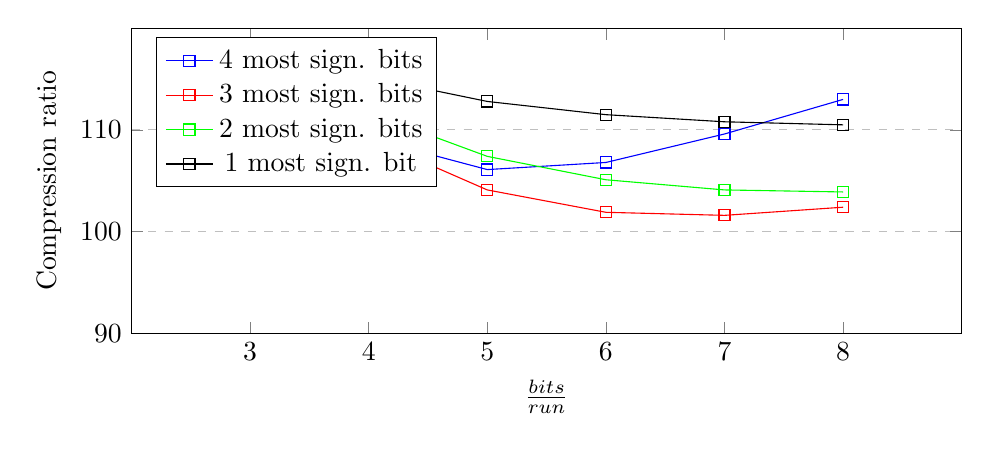
\begin{tikzpicture}%[scale=\tikzscale]
\begin{axis}[
width=\textwidth,
height=0.45\textwidth,
xlabel={$\frac{bits}{run}$},
ylabel={Compression ratio},
xmin=2, xmax=9,
ymin=90, ymax=120,
xtick={3,4,5,6,7,8},
ytick={90,100,110},
legend pos=north west,
ymajorgrids=true,
grid style=dashed,
]
\addplot[
	color=blue,
	mark=square,
	]
	coordinates {
		(4,109.2)(5,106.1)(6,106.8)(7,109.6)(8,113)
	};
\addplot[
	color=red,
	mark=square,
	]
	coordinates {
		(4,109.2)(5,104.1)(6,101.9)(7,101.6)(8,102.4)
	};
\addplot[
	color=green,
	mark=square,
	]
	coordinates {
		(4,111.7)(5,107.4)(6,105.1)(7,104.1)(8,103.9)
	};
\addplot[
	color=black,
	mark=square,
	]
	coordinates {
		(4,115.2)(5,112.8)(6,111.5)(7,110.8)(8,110.5)
	};
	\legend{4 most sign. bits,3 most sign. bits,2 most sign. bits, 1 most sign. bit}
\end{axis}
\end{tikzpicture}
%}
%\end{scaletikzpicturetowidth}
\caption{Different run lengths for byte mapping and varying maximum run lengths}
\label{fig:2:different run lengths for byte mapping and varying maximum run lengths}
\end{figure}

\par{
The combination of 3 bits per run and 7 bits per run for the 3 most significant bits yielded the overall best results with 101.6\% of its original size and 8.13 $\frac{bits}{symbol}$ as shown in Figure \ref{fig:2:different run lengths for byte mapping and varying maximum run lengths}. It has to be mentioned, that the expected overhead is rather small but the increase in average run length lead to a reduction in size which was still not really compressing. Some files got a little smaller while other files almost doubled in size which is still no real enhancement over regular rle which performs really well on specific files.
\begin{table}[H]
	\centering
	\begin{tabular}{r|r|r|r|r}	
		file & size original & size encoded & ratio in \% & $\frac{bits}{symbol}$\\
		\hline
		bib & 111261 & 97867 & 87.96 & 7.03\\
		book1 & 768771 & 579649 & 75.39 & 6.03 \\
		book2 & 610856 & 484989 & 79.39 & 6.35\\
		geo & 102400 & 116487 & 113.75 & 9.10\\
		news & 377109 & 315446 & 83.64 & 6.69\\
		obj1 & 21504 & 23871 & 111.00 & 8.88\\
		obj2& 246814 & 276301 & 111.94 & 8.95\\		 
		paper1 & 53161 & 43556 & 81.93 & 6.55\\		 
		paper2& 82199 & 62544 & 76.08 & 6.08\\		 
		pic & 513216 & 272034 & 53.00 & 4.24\\		 
		progc & 39611 & 33073 & 83.49 & 6.67\\		 
		progl & 71646 & 53653 & 74.88 & 5.99\\		 
		progp & 49379 & 39400 & 79.79 & 6.38\\		 
		trans & 93695 & 84494 & 90.17 & 7.21\\
		\hline
		all files & 3145718 & 2487460 & 79.07 & 6.32
	\end{tabular}
	\caption{Calgary Corpus encoded with vertical reading, byte remapping and 2 bits per RLE run and 5 for the 3 most significance bits}
\label{tab:t43 Calgary Corpus encoded with vertical reading, byte remapping and 2 bits per RLE run and 5 for the 3 most significance bits}
\end{table}

2020-01-13 21:39:50 INFO/Analyzer  Corpus size original: 3145718 // 3.145718 Mb  
2020-01-13 21:39:50 INFO/Analyzer  Corpus size encoded: 3197179 // 3.197179 Mb  
2020-01-13 21:39:50 INFO/Analyzer  1.0163590633362558 compression ratio  
2020-01-13 21:39:50 INFO/Analyzer  with 8.130872506690046 bits/symbol  
2020-01-13 21:39:50 INFO/Analyzer  File bib, size original: 111261, size encoded: 127820, compression: 114.8830228022398, bps: 9.190641824179183  
2020-01-13 21:39:50 INFO/Analyzer  File book1, size original: 768771, size encoded: 735120, compression: 95.62275371989838, bps: 7.64982029759187  
2020-01-13 21:39:50 INFO/Analyzer  File book2, size original: 610856, size encoded: 623881, compression: 102.13225375538588, bps: 8.17058030043087  
2020-01-13 21:39:50 INFO/Analyzer  File geo, size original: 102400, size encoded: 159874, compression: 156.126953125, bps: 12.49015625  
2020-01-13 21:39:50 INFO/Analyzer  File news, size original: 377109, size encoded: 407185, compression: 107.97541294426811, bps: 8.638033035541449  
2020-01-13 21:39:50 INFO/Analyzer  File obj1, size original: 21504, size encoded: 31871, compression: 148.20963541666669, bps: 11.856770833333334  
2020-01-13 21:39:50 INFO/Analyzer  File obj2, size original: 246814, size encoded: 369726, compression: 149.7994441158119, bps: 11.983955529264952  
2020-01-13 21:39:50 INFO/Analyzer  File paper1, size original: 53161, size encoded: 56323, compression: 105.94796937604636, bps: 8.475837550083709  
2020-01-13 21:39:50 INFO/Analyzer  File paper2, size original: 82199, size encoded: 79621, compression: 96.86370880424336, bps: 7.749096704339469  
2020-01-13 21:39:50 INFO/Analyzer  File pic, size original: 513216, size encoded: 330347, compression: 64.36802437959845, bps: 5.149441950367876  
2020-01-13 21:39:50 INFO/Analyzer  File progc, size original: 39611, size encoded: 42454, compression: 107.17729923506096, bps: 8.574183938804877  
2020-01-13 21:39:50 INFO/Analyzer  File progl, size original: 71646, size encoded: 68051, compression: 94.98227395807163, bps: 7.59858191664573  
2020-01-13 21:39:50 INFO/Analyzer  File progp, size original: 49379, size encoded: 50333, compression: 101.93199538265254, bps: 8.154559630612203  
2020-01-13 21:39:50 INFO/Analyzer  File trans, size original: 93695, size encoded: 110477, compression: 117.91130796734083, bps: 9.432904637387267 
}

\subsection{Burrows-Wheeler-Transformation Appliance}
\par{
Another possible preprocessing step which promised an improvement is the mentioned Burrows-Wheeler-Transformation from Section \ref{ch:Principles of compression:sec:Other:subSec:bwt}, initially applied to regular binary and byte wise RLE. By mistake a very simple transformation implementation was chosen, working by adding additional start and stop symbols to the input string (0x02 as STX, start of text and 0x03 as ETX, end of text). Some basic testing and playing around worked great but later on it revealed some major issues. For example the Calgary Corpus consists of more than textual data, in fact the files geo, obj1, obj2 and pic contain of some binary data of include the symbols STX or ETX so we wont be able to apply the transformation to these. Another shortcoming was the very poor time complexity of almost $O (n^2)$ because under the hood, it uses a dual pivot Quick-sort algorithm from the JDK 11, which is typically faster than traditional one pivot Quick-sort. This algorithm offers $\Theta (n \: log(n))$ average time complexity but in the worst case, its time complexity is cubic. This problem was partially solved by reading the input data in parts and performing the transformation on each part, result in a much smaller length $n$ and thus better run time at the expense of a slightly worse transformation result. As all chunks are individual transformations, they can also be computed in parallel without much effort.

\begin{table}[H]
	\centering
	\begin{tabular}{r|r|r}	
		bits per rle number & ratio in \% & bits per symbol in $\frac{bits}{symbol}$\\
		\hline
		3 & 95.41 & 7.63\\
		2 & 91.39 & 7.31 \\
	\end{tabular}
	\caption{Initial BWT implementation on byte wise RLE}
	\label{tab:t11 Simple Burrows Wheeler Transformation on byte wise RLE}
\end{table}
}
\par{
While it was only applicable to textual data and very slow, even when divided into smaller parts and computed in parallel, it improved the overall results of byte wise RLE by 16\% to a compression ratio of slightly over 7 $\frac{bits}{symbol}$ which seemed like a good start. Regular binary RLE did not really benefit from this transformation as expected but on vertical interpretation, consecutive characters result in successive bits on every significance. Still this implementation had to be dropped and switched against one that could handle arbitrary input to be able to transform all files. This time all files could be processed and the resulting compression with byte wise RLE improved further.

\begin{table}[H]
	\centering
	\begin{tabular}{r|r|r}	
		bits per rle number & ratio in \% & bits per symbol in $\frac{bits}{symbol}$\\
		\hline
		3 & 91.62 & 7.33\\
		2 & 89.46 & 7.15
	\end{tabular}
	\caption{Burrows Wheeler Transformation on byte wise RLE}
	\label{tab:t12 Burrows Wheeler Transformation on byte wise RLE}
\end{table}
}

\par{
In Section \ref{ch:Principles of compression:sec:Other} the Burrows-Wheeler-Transformation inversion was performed using a Matrix M containing all cyclic rotations of the input word, sorted in lexicographic order. However this is has a bad complexity and the inverting process does not even has access to this Matrix M.\\

TODO: explain creation using suffix array \\
}

\par{
In general a Burrows-Wheeler-Transformation should also increase the runs in the implementation of Section \ref{ch:Analysis:sec:Improvements by Preprocessing:subSec:vertReading} and \ref{ch:Analysis:sec:Improvements by Preprocessing:subSec:byteRemapping} so those preprocessing steps were also applied in combination. To do so, it was first swapped against an sufficient implementation provided by a paper from m. Burrows and D. J. Wheeler \cite{Burrows94} from 1994. Their method is also the one described in Section \ref{ch:Analysis:sec:Improvements by Preprocessing:subSec:bwt} and could handle arbitrary input but it also had some downsides like the additional index $I$ of the transformation, which had to be persisted as well. The major downside of this implementation although was the rather slow. To overcome this issue and the saving of additional indices, the implementation used had to be swapped once more against one that was first described by \cite{Burrows-linear-time} in 2009.

TODO: explain inversion using Lyndon words
}
\par{
Swapping the implementation resulted in way better results, even with the simple regular RLE archiving compression ratios around 60 \% of its original size was possible while using 4 bits per run. This was mainly because of the longer repetitions possible after the transformation was performed on the whole input instead of small chunks. Another reason is the lack of additional information needed to store because we do no longer need to store the transformation index of every chunk.
	\begin{table}[H]
		\centering
		\begin{tabular}{r|r|r}	
			bits per rle number & ratio in \% & bits per symbol in $\frac{bits}{symbol}$\\
			\hline
			8 & 74.5 & 5.96\\
			7 & 70.0 & 5.60\\
			6 & 65.7 & 5.25\\
			5 & 61.8 & 4.98\\
			4 & 59.9 & 4.81\\
			3 & 61.3 & 4.94\\
			2 & 69.8 & 5.42
		\end{tabular}
		\caption{Modified Burrows Wheeler Transformation on byte wise RLE}
		\label{tab:t12 Modified Burrows Wheeler Transformation on byte wise RLE}
	\end{table}
}


\par{
Using the modified bijective Burrows-Wheeler-Transformation, regular binary and byte-wise RLE had their peak performance while using 4 bits per encoded number but interestingly the vertical encoded RLE did not. Instead it maxed out with 4 bits per encoded number with 67 \% of its original size with only 5.42 $\frac{bits}{symbol}$. Combining the byte mapping and the transformation yielded slightly better results with 65 \% and 5.22 $\frac{bits}{symbol}$ as show in Figure \ref{fig:3:Different run lengths with and without transformations}. There was still room for some optimizations because as seen in Section \ref{ch:Conceptual Design:sec:var lengths}, the remapping of the input resulted in longer runs on the higher order bits and the vertical interpretation made it possible to encode different sections with different maximum run lengths.

TODO: make both plots align side by side
\begin{figure}[H]
	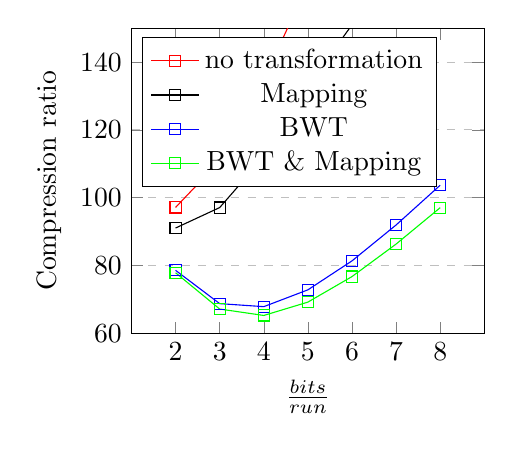
\begin{tikzpicture}[scale=1]
	\begin{axis}[
	width=.5\textwidth,
	height=0.45\textwidth,
	xlabel={$\frac{bits}{run}$},
	ylabel={Compression ratio},
	xmin=1, xmax=9,
	ymin=60, ymax=150,
	xtick={2,3,4,5,6,7,8},
	ytick={60,80,100,120,140},
	legend pos=north west,
	ymajorgrids=true,
	grid style=dashed,
	]
	\addplot[
	color=red,
	mark=square,
	]
	coordinates {
		(2,97.14)(3,110.82)(4,134.83)(5,163)(6,192)
	};
	\addplot[
	color=black,
	mark=square,
	]
	coordinates {
		(2,91.06)(3,97.1)(4,112)(5,133)(6,151)
	};
	\addplot[
	color=blue,
	mark=square,
	]
	coordinates {
		(2,78.58)(3,68.76)(4,67.87)(5,72.83)(6,81.37)(7,91.96)(8,103.69)
	};
	\addplot[
	color=green,
	mark=square,
	]
	coordinates {
		(2,77.87)(3,67.17)(4,65.27)(5,69.21)(6,76.74)(7,86.33)(8,97.07)
	};
	\legend{no transformation,Mapping,BWT,BWT \& Mapping}
	\end{axis}
	\end{tikzpicture}
	\caption{Different run lengths with and without transformations}
	\label{fig:3:Different run lengths with and without transformations}
	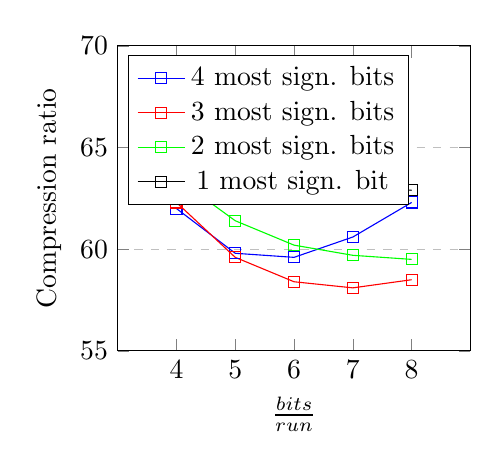
\begin{tikzpicture}[scale=1]
	\begin{axis}[
	width=.5\textwidth,
	height=0.45\textwidth,
	xlabel={$\frac{bits}{run}$},
	ylabel={Compression ratio},
	xmin=3, xmax=9,
	ymin=55, ymax=70,
	xtick={4,5,6,7,8},
	ytick={55,60,65,70},
	legend pos=north west,
	ymajorgrids=true,
	grid style=dashed,
	]
	\addplot[
	color=blue,
	mark=square,
	]
	coordinates {
		(4,62)(5,59.8)(6,59.6)(7,60.6)(8,62.3)
	};
	\addplot[
	color=red,
	mark=square,
	]
	coordinates {
		(4,62.3)(5,59.6)(6,58.4)(7,58.1)(8,58.5)
	};
	\addplot[
	color=green,
	mark=square,
	]
	coordinates {
		(4,63.5)(5,61.4)(6,60.2)(7,59.7)(8,59.5)
	};
	\addplot[
	color=black,
	mark=square,
	]
	coordinates {
		(4,65.2)(5,64.1)(6,63.4)(7,63.0)(8,62.9)
	};
	\legend{4 most sign. bits,3 most sign. bits,2 most sign. bits, 1 most sign. bit}
	\end{axis}
	\end{tikzpicture}
	\caption{Different run lengths for byte mapping and transformation and varying maximum run lengths}
	\label{fig:4:Different run lengths for byte mapping and transformation and varying maximum run lengths}
\end{figure}
}

\par{
In Section \ref{ch:Conceptual Design:sec:var lengths} different run lengths for different significant bits provided an edge over just fixed maximum run length, so this combination was also tried out. After testing all combinations of possible and reasonable variables it was found that using a Burrows-Wheeler-Transformation and byte remapping as preprocessing steps, parse the transformed data in vertical order and then using 3 bits per run for low significant bits and 7 for the 3 most significant bits, run length encoding performs at its peak. Using this setup, the Calgary Corpus can be compressed down to 58.1 \% of its original size while using only 4.65 $\frac{bits}{symbol}$ as shown in figure \ref{fig:4:Different run lengths for byte mapping and transformation and varying maximum run lengths}. This was the best result achieved so far and the detailed compression results are shown below.

TODO: reevaluate results after bug!!!
\begin{table}[H]
	\centering
	\begin{tabular}{r|r|r|r|r}	
		file & size original & size encoded & ratio in \% & $\frac{bits}{symbol}$\\
		\hline
		bib & 111261 & 62791 & 56.43 & 4.51\\
		book1 & 768771 & 465661 & 60.57 & 4.84 \\
		book2 & 610856 & 343998 & 56.31 & 4.51\\
		geo & 102400 & 117428 & 114.67 & 9.17\\
		news & 377109 & 232600 & 61.67 & 4.93\\
		obj1 & 21504 & 22242 & 103.43 & 8.27\\
		obj2& 246814 & 180879 & 73.28 & 5.86\\		 
		paper1 & 53161 & 31608 & 59.45 & 4.75\\		 
		paper2& 82199 & 46982 & 57.15 & 4.57\\		 
		pic & 513216 & 196148 & 38.21 & 3.05\\		 
		progc & 39611 & 24186 & 61.05 & 4.88\\		 
		progl & 71646 & 33233 & 46.38 & 3.71\\		 
		progp & 49379 & 23753 & 48.10 & 3.84\\		 
		trans & 93695 & 44203 & 47.17 & 3.77\\
		\hline
		all files & 3145718 & 1829808 & 58.16 & 4.65
	\end{tabular}
	\caption{Calgary Corpus encoded, all preprocessing steps, using 3 bits per RLE run and 7 for the 3 most significance bits}
	\label{tab:t5:Calgary Corpus encoded, all preprocessing steps, using 3 bits per RLE run and 7 for the 3 most significance bits}
\end{table}
\par{
One last option was the encoding of the lowest significant bits with another, more suited scheme like Huffman encoding was tried out but with rather poor results. It was found that encoding the last or the last few rows seen in \ref{ch:Analysis:sec:Improvements by Preprocessing:subSec:vertReading} with did not improve overall results and it was therefore discarded. This might be related to the high improvement in RLE after a Burrows-Wheeler-Transformation and other factors like additional overhead because the mapping of the Huffman encoding has to be persisted with the encoded data. But the idea of combing the RLE methods with Huffman encoding still stuck around and was picked up again later on in a modified way in Section \ref{ch:Conceptual Design:sec:Postprocessing}. No further attempts to add or improve preprocessing steps of this kind were made, instead the results were analyzed and compared with other results in section \ref{ch:Evaluation}.
}
%% ==============================
\section{Other Processing Options}
%% ==============================
\label{ch:Conceptual Design:sec:Postprocessing}
Another step worth mentioning was the encoding using Huffman codes after the Run length encoding was performed, similar to the Fax Transmission Standard mentioned in section \ref{ch:Principles of compression:sec:Run Length Encoding:subSec:History}, but i a dynamic way instead of predefined static codes. This idea was also used by Burrows and Wheeler in their paper \cite{Burrows94} but instead of RLE they combined a Move to Front Coder with their transformation and then encoded the result using Huffman codes. This way it would be possible to encode more frequent results of the Move to Front Encoder or the Run Length Encoder could be encoded into shorter codes and thus save even more space. However this step is not considered preprocessing anymore but could improve the compression furthermore.

\subsection{Performance improvements}
TBD
%% ==============================
\section{Implementation Decisions}
%% ==============================
\label{ch:Conceptual Design:sec:Implementation Decisions}

The algorithms described have all been implemented using Kotlin, because it can be compiled for the Java Virtual Machine as well as native, so it seemed like a good balance between native speed and higher language conciseness and fault-tolerance. Also there were some library available for Byte- and Bit-Operations on streams which proved to be quite useful.

%% ==============================
\section{Implementation Detail}
%% ==============================
\label{ch:Conceptual Design:sec:Implementation Detail}
- detailed information about specific modules and classes\\
\ldots

\subsection{Burrows Wheeler Transformation}
- TBD\\
\subsection{Byte Remapping}
- show use case \\

%% ==============================
\section{Implementation Evaluation}
%% ==============================
\label{ch:Conceptual Design:sec:Implementation Evaluation}
- evaluation of implementation choices made


%% ==============================
\section{Summary}
%% ==============================
\label{ch:Conceptual Design:sec:Summary}

Am Ende sollten ggf. die wichtigsten Ergebnisse nochmal in \emph{einem}
kurzen Absatz zusammengefasst werden.

%%% Local Variables: 
%%% mode: latex
%%% TeX-master: "thesis"
%%% End: 
     % Entwurf
\chapter{Implementation}
\label{ch:Implementation}
%% ==============================
All algorithms described have been implemented using Kotlin, because it can be compiled for the Java Virtual Machine as well as native, so it seemed like a good balance between a native implementation and higher language conciseness and fault-tolerance. Also there were some libraries available for byte and bit operations on streams which proved to be quite useful, although there was almost no documentation available. This one and all other libraries are described in section \ref{ch:Implementation:sec:Impl:subsec:libs}. The main focus is on the encoder and decoder classes but the other modules will be discussed as well. The project is realized as a maven project, to simplify dependency management. 

\section{Binary and byte wise RLE}
\label{ch:Implementation:bin and byte rle}
\par{
	The simple binary and byte wise RLE are rather trivial and implemented together in one encoder, the \textit{StringRunLengthEncoder}. The binary version is implemented with the mentioned BitStream from the IOStreams library. It allows working on a stream and reading and writing bit by bit and also reading the next n bit as signed or unsigned number which comes in handy during decoding. In general, it is called with a variable $b$ bitsPerRun which sets the used bits to store one run. At first a maximum run length is determined by the maximum value $b$ can store as a binary string, $l(b) = n$ implies a maximum value of $2^{n-1}$. Then the input is read consecutively in bits and the runs of equal bits are counted. We are always assuming the run starts with zero, if this is not the case a leading run of 0 is added, which means there are zero times 0 at the beginning. If a run exceeds the maximum run length, the maximum is written and again an artificial zero is added to the output stream to signal a length higher than the maximum. Each run can simply be written to the output stream with the desired amount of bits per run. During decoding, we assume the same $b$ and can then always read $n$ bits of the stream as unsigned value, know each run again and can therefore reconstruct the original data.
}
\par{
	Byte wise RLE is working with a similar idea of counting $n$ runs of equal information. This time it is applied on a byte level, reading byte after byte. If the next byte is the same as the current one, the counter is incremented, if not the run and the byte value are encoded as pair $(n, byte)$ to the output. The byte value itself still needs 8 bit of information but the run does not. Most raw untreated data does not contain long runs of consecutive identical byte values average run length is rather small. This implied storing a count of 1 or 2 in 8 bits of space which in turn explained the expansion in size seen in table \ref{tab:t31 Byte-wise RLE on the Calgary Corpus}. Therefore this version was also implemented with an arbitrary amount of bits to save per run, to minimize the overhead. If a run exceeds the maximum, which is again determined by the amount of bits stored per run, it is encoded twice, once with the maximum count and once with the remaining count. We do not need a zero run in this version because we also store the value itself, therefore we can count without a zero. This means for an example run of 4 times the value \textit{0xFF} and 4 bits per run saved, it will be encoded as the pair $(0011,0xFF)$ or $001111111111$ as consecutive binary stream.
}
\section{Vertical binary RLE}
\label{ch:Implementation:vertical rle}
\par{
	Basically the ideas described in sections \ref{ch:Analysis:sec:Improvements by Preprocessing:subSec:vertReading} and \ref{ch:Conceptual Design:sec:Parallel Byte Reading} oppose only a small variance compared to regular binary RLE. It is realized with the use of BitStreams again. Its stream interface offers a position $p$, which corresponds to the byte value and a offset $o$, which is a bit value with significance $o$ of byte $p$, which allows reading all bits of the same significance in order. This was done for significance zero to seven to read all bits in a vertical manner as in the examples. Then each run is again counted with the same method including a maximum run length defined by the amount of bits used to count a run and the runs are then written with the fixed amount of bits to the output stream. Afterwards, the amount of runs per bit position is written to the tail of the encoded file, without the information how many runs are expected it would be much more difficult to decide which run belongs where, but it is still possible. The average overhead of this additional information is around 34 byte, two for each count and a two byte stop symbol which is only needed seven times, no additional stop at the end of the file. Even though it was originally designed to work on chunks of bytes, in the end the transformations worked on the file or on the stream itself, which was significantly faster.
}
\par{
	During decoding, the expected amount of runs are parsed from the end of the file. Then the actual decoding happens, with the fixed $n$ bits per code for this bits significance. Knowing the exact amount of RLE numbers for each bit position makes it easy to decode, because the variable length of encoded numbers can be chosen accordingly while reading the stream once. Assuming a starting run on zero, all runs are written back to one file, each bit position sequentially, to then assemble the original data. This is done for each bit position in sequential order so we need to write 8 times to the output file. It might be worth trying out building the byte stream in memory and the write the output only once, which might be faster but also requires more internal data structures and holding the whole file in memory at once.
}
\section{Byte Remapping}
\label{ch:Implementation:bytemapping}
\par{
	To start of with the preprocessing, the byte remapping was implemented. The \emph{Analyzer} is responsible for generating a overall probability distribution over the values of bytes contained in the file. This serves as a input for the map generation, where every byte value is sorted accordingly to its occurrence and mapped to increasing byte values, so the most frequent byte to \textit{0x00}, the second most often to \textit{0x01} and so on. Afterwards, a temporary file is generated where each byte from the original file is mapped, which allows streaming during the encoding process. Decoding requires access to the original mapping, therefore it is persisted at the start of the encoded file. To do so, we only need to know the number of mapped values and then the original byte, not the mapped value since we know they are sorted acceding.
}
\section{Burrows Wheeler Transformation}
\label{ch:Implementation:bwt}
\par{
	As mentioned earlier, the Burrows-Wheeler-Transformation is implemented in 3 different versions, starting of with the naive vs.\ unsophisticated. The \emph{transformation.BurrowsWheelerTransformation} is implemented with the use of start and stop symbols (0x02 as STX and 0x03 as ETX) and with the creating and sorting of all cyclic rotations of the input string. This can be done for all text input files but not for binary data because files containing the start or stop symbols confused the algorithm and made the inverse transformation impossible. Additionally it is extremely slow due to its at least quadratic complexity, even when working on small chunks which messes up the overall transformation result. It is not further described as it was only used for some initial testing to see if and how much RLE benefits from this transformation. 
}
\par{
	The second implementation is realized by following the original algorithm description provided in greater detail in the paper by M. Burrows and D. J. Wheeler \cite{Burrows94} (algorithm C and D). The \emph{transformation.BurrowsWheelerTransformationModified} works on parts of the data so the transformation result is still strongly depending on the size of the chunks, but it could at least handle arbitrary input. Higher chunk sizes greatly increased the transformation because more equal characters are in the same chunk but also really slowed down the process. Due to fact that both the mapping and the modified transformation work on an array of bytes and do not interfere with one-another, they can be performed in any order. The further on used advanced implementation of the bijective Burrows-Wheeler-Scott-Transformation is ported from Java from an external source or directly usable as dependency and therefore described in section \ref{ch:Implementation:sec:Impl:subsec:libs}.
}
\section{Huffman encoding}
\label{ch:Implementation:Huffman}
\par{
Following the pseudo-code provided by M. Liśkiewicz and H. Fernau in \cite{entropy-fernau} on page 21 the implementation was straight forward. Internally a small set of data structures are provided for assembling the Huffman tree, a \emph{HuffmanTree}, a \emph{HuffmanNode} and a \emph{HuffmanLeaf} class is implemented. The HuffmanTree is abstract and only holds the frequency of a tree, since every tree itself has its own frequency. It also implements a compareTo function, to draw comparisons between different trees. A HuffmanNode extends the HuffmanTree, consists of a left and right HuffmanTree and has their sum of frequencies as frequency. The leaf is itself also a tree and holds a value of type byte and a frequency which resembles its occurrence. To build the Huffman tree for a given set of bytes, the algorithm expects an array of integer $I$, assembling the occurrences $o$ of bytes $b \in [ 0,255 ]$ in the form of $I [ b ] = o$. Then a leaf is created for every entry of $I$ with a frequency of $o$ and collected into a PriorityQueue of HuffmanTrees. Then while there are still at least two trees left in the queue, the two lowest frequencies are removed from the queue, merged into a single tree and reinserted into the queue. After the creation of the tree, all paths are followed and every time a leaf is reached, the current path is added to a map in form of a StringBuffer $b$. This buffer contains the path of left and right trees traversed into the original one, adding a zero for every left descent and a one for every right one. Finally the mapping of type byte to StringBuffer is returned. To apply this algorithm to the runs of the RLE encoding, the same is done except that instead byte values, every possible run length value is counted and collected into the same structure.
}
\par{
To reverse this Huffman coding it is required to have access to the performed mapping, otherwise decoding would be impossible. Therefore the map itself is written to the beginning of the file, similar to the mapping from section \ref{ch:Implementation:bytemapping}. This time though we need triplets of values, because the Huffman code can have a variable length, so the mapping is encoded to $(b,l(b),b)$, with $b$ and $l(b)$ each assuming one byte. This also implies a maximum length for Huffman codes of 255. During decoding of the mapping, first the total number of mappings is parsed. Then while there are still more mappings expected, we parse one byte which is the mapping value, then one byte which contains the length of the following mapping as unsigned byte value and then the Huffman code of the given length is parsed bit by bit and saved as a StringBuffer. This way it is possible to write and read the variable length codes continuously from the stream. 
}
\section{External libraries}
\label{ch:Implementation:sec:Impl:subsec:libs}
\par{
Some external libraries are used in throughout this project. Most of them provide a set of sealed functionality, like \emph{io.github.jupf.staticlog} which just facilitate the logging features and are not further interesting, therefore most of them are mention in section \ref{ch:Implementation:sec:Impl:subsec:libs:others}, only extensively used ones are described in greater detail. 
}

\subsection{IOStreams for Kotlin}
\label{ch:Implementation:sec:Impl:subsec:libs:iostreams}
\par{
Alexander Kornilov created and released this library, which was found in the \href{https://discuss.kotlinlang.org/t/i-o-streams-for-kotlin/9802}{Kotlin forum}} and is currently hosted on \href{https://sourceforge.net/projects/kotlin-utils/}{Sourceforge}. It has a very light documentation \cite{IoStreamsKotlin} and is released with an Apache v2.0 license. It has to be mentioned that for the time being there is only a pre-release available, this version 0.33 is used throughout this project. Moving to this library rendered it possible to work entirely on streams of data as well as reading the next $n$ bit(s). This greatly improved the performance of the initial algorithm and reduced required data structures and memory. There was also some odd or unexpected behavior seen which might be changed in further versions, for example if the stream is currently at the first byte and we want to write to its bit with the highest significance. This represents a so called bit offset of 7, so we can write the position as 0:7. Writing a 1 or setting this bit to true advances the position of the stream to the next byte and offset zero, so 1:0 while writing a 0 keeps the stream at its current position so it is still at 0:7 and the next bit gets written on the same position. Basically the interface provides good functionality with the drawback of some inconsistencies.
}

\subsection{libDivSufSort}
\label{ch:Implementation:sec:Impl:subsec:libs:libDivSufSot}
\par{
The original code for the modified BWTS algorithm and the necessary sorting algorithms called \emph{DivSufSort} for efficient suffix array sorting was provided by Yuta Mori in the library \href{https://github.com/y-256/libdivsufsort}{libDivSufSort} \cite{LibDivSufSort} and is as already mentioned, closer described in the paper by Johannes Fischer and Florian Kurpicz \cite{DBLP:journals/corr/abs-1710-01896}. It  runs in $O(n log n)$ worst-case time using only $5n+O(1)$ bytes of memory space, where $n$ is the length of the input. The code is available under the MIT license at Github but written in C and thus, rather hard to use from Kotlin. Further research lead to a port to Java which uses the same structures and methods but is already close to the desired state, since Kotlin enables using Java classes by default.
}
\subsection{libDivSufSort in Java}
\label{ch:Implementation:sec:Impl:subsec:libs:libDivSufSort Java}
\par{
Porting the Java implementation provided by \href{https://github.com/flanglet/kanzi/releases}{kanzi} \cite{kanzi}, a collection of state of the art compression methods, all available in Java, C++ and Go, was easy but also gratuitous, since there are releases available for the Java version which is still maintained at a high frequency. To use them we simply add the dependency to our maven project. This library basically provides one functionality, the implementation of a sophisticated bijective Burrows-Wheeler-Scott-Transformation in linear time.
}
\par{
To skim over its functionality, it provides a clean API to work with advanced compression algorithms in Java, most noticeable \emph{DivSufSort} and \emph{BWTS}. The BWTS class offers just the two directions of the transformation as methods, both working on arrays of bytes, which requires reading all the input into memory. This functionality is encapsulated by the class \emph{BWTSWrapper} to work on file level and generate a temporary file with the transformed contents to further work on a stream of that file. At first the whole input is spliced into Lyndon words. Then the suffix array is generated and sorted, using the fastest known suffix sorting algorithm DivSufSort. The result is also written to a temporary file, like the mapping which was quite useful for debugging, and enables streaming its contents during encoding. 
}

\subsection{Others}
\label{ch:Implementation:sec:Impl:subsec:libs:others}
\par{
Besides logging, some other basic functionality was added which was quite simple through the use of maven. \emph{org.junit.jupiter} provided the packages \emph{junit}, \emph{engine} and \emph{api} in version 5.6.0, which allows a simple test unit creation and execution. Additionally \emph{assert-j} in version 3.13.2 added extended assertion capabilities to the encoder as well as to the test cases. A modest approach of multithreading was enabled by use of Kotlin \emph{coroutines} in version 1.3.2, provided by Jetbrains. Just by convenience, Googles \emph{guava} was used in version 28.2 for new collection types and a comparator for an array of bytes.
}


%% ==============================
\section{Implementation Evaluation}
%% ==============================
\label{ch:Implementation:sec:Implementation Evaluation}
\par{
Obviously the assembled tool does not compete with the state of the art methods used today, neither in comparison of their compression results nor in terms of speed. There is most likely still a lot of unused potential to speed things up, for example by excessive multithreading. Also, decoding could be vastly speed up by writing each output byte only once instead of up to 8 times if the byte is of value 0xFF. Even compression results could probably be further improved but more on that in chapter \ref{ch:Discussion}. Nonetheless, the desired concept was proven and the results show a clear advantage over regular RLE achieved through preprocessing. 
}

%% ==============================
\section{Usage}
%% ==============================
\label{ch:Implementation:sec:usage}
\par{
To enable a convenient usage, the algorithm is obtainable as jar file but it can also be built from sources. It provides a simple command line interface which expects a desired action, either compressing \emph{-c} or decompressing \emph{-d} and a method, either vertical RLE \emph{-v}, binary \emph{-bin} or byte wise RLE \emph{-byte}. Binary and byte wise RLE can optionally be called with a parameter $N$ where $N$ is the amount of bits used to encode a single RLE number, vertical encoding can also run with an arbitrary amount of bits, but expects 8 comma separated numbers \emph{-v N,N,N,N,N,N,N,N}. As preprocessing options, mapping \emph{-map}, applying the sophisticated Burrows-Wheeler-Transformation \emph{-bwt} and Huffman encoding \emph{-huf} are available via the parameters. Additional information can be acquired by launching the application with \emph{-h} for further help. To enable debug logging and get detailed insight into the compression and decompression steps, the parameter \emph{-D} has to be set.
}

%%% Local Variables: 
%%% mode: latex
%%% TeX-master: "thesis"
%%% End: 
    % Implementierung
%% eval.tex
%% $Id: eval.tex 61 2012-05-03 13:58:03Z bless $

\chapter{Evaluation}
\label{ch:Evaluation}
%% ==============================
Hier erfolgt der Nachweis, dass das in Kapitel~\ref{ch:Conceptual Design}
entworfene Konzept funktioniert. 
Leistungsmessungen einer Implementierung werden immer gerne gesehen.

%% ==============================
\section{Functional Evaluation}
%% ==============================
\label{ch:Evaluation:sec:Functional Evaluation}
- Mathematical Comparison\\
- Comparison of encoded file sizes\\
- comparing to regular REL and Huffman coding\\
\ldots

%% ==============================
\section{Benchmarks}
%% ==============================
\label{ch:Evaluation:sec:Benchmarks}
- Benchmark with the Galgary corpus\\
\url{http://www.data-compression.info/Corpora/} \\
\ldots

%% ==============================
\section{Conclusion}
%% ==============================
\label{ch:Evaluation:sec:Conclusion}

Am Ende sollten ggf. die wichtigsten Ergebnisse nochmal in \emph{einem} kurzen Absatz zusammengefasst werden.

%%% Local Variables: 
%%% mode: latex
%%% TeX-master: "thesis"
%%% End: 
        % Evaluation
%% zusammenf.tex
%% $Id: zusammenf.tex 61 2012-05-03 13:58:03Z bless $
%%

\chapter{Discussion}
\label{ch:Discussion}
%% ==============================

- use other probability approach\\
- use huffman for byte wise rel and bwt\\

%%% Local Variables: 
%%% mode: latex
%%% TeX-master: "thesis"
%%% End: 
   	  % Diskussion und Ausblick

%% ++++++++++++++++++++++++++++++++++++++++++
%% Anhang
%% ++++++++++++++++++++++++++++++++++++++++++

\appendix
%\include{anhang_a}
%\include{anhang_b}

%% ++++++++++++++++++++++++++++++++++++++++++
%% Literatur
%% ++++++++++++++++++++++++++++++++++++++++++
%  mit dem Befehl \nocite werden auch nicht 
%  zitierte Referenzen abgedruckt

\cleardoublepage
\phantomsection
\addcontentsline{toc}{chapter}{\bibname}
%%
%%\nocite{*} % nur angeben, wenn auch nicht im Text zitierte Quellen 
           % erscheinen sollen
%\bibliographystyle{itmabbrv} % mit abgekürzten Vornamen der Autoren
\bibliographystyle{plain} % abbrvnat unsrtnat
% spezielle Zitierstile: Labels mit vier Buchstaben und Jahreszahl
%\bibliographystyle{itmalpha}  % ausgeschriebene Vornamen der Autoren

\bibliography{thesis}

%% ++++++++++++++++++++++++++++++++++++++++++
%% Index
%% ++++++++++++++++++++++++++++++++++++++++++
\ifnotdraft{
\cleardoublepage
\phantomsection
\printindex            % Index, Stichwortverzeichnis
}

 %
 % Die folgende Erklärung ist für Diplomarbeiten Pflicht
 % (siehe Prüfungsordnung), für Studienarbeiten nicht notwendig
 \thispagestyle{empty}
%\vspace*{35\baselineskip}
%\hbox to \textwidth{\hrulefill}
\par
\chapter*{Eidesstattliche Erklärung}

Hiermit erkläre ich, dass ich diese Bachelor-/Masterarbeit selbständig verfasst und keine anderen als die angegebenen Quellen und Hilfsmittel benutzt und die aus fremden Quellen direkt oder indirekt übernommenen Gedanken als solche kenntlich gemacht habe. Die Arbeit habe ich bisher keinem anderen Prüfungsamt in gleicher oder vergleichbarer Form vor-gelegt. Sie wurde bisher auch nicht veröffentlicht.

Trier, den xx. Monat 20xx

%%%%%%%%%%%%%%%%%%%%%%%%%%%%%%%%%%%%%%%%%%%%%%%%%%%%%%%%%%%%%%%%%%%%%%%%
%% Hinweis:
%%
%% Diese Erklärung wird von der Prüfungsordnung für Diplomarbeiten 
%% verlangt und ist zu unterschreiben. Für Studienarbeiten ist diese
%% Erklärung nicht zwingend notwendig, schadet aber auch nicht.
%%%%%%%%%%%%%%%%%%%%%%%%%%%%%%%%%%%%%%%%%%%%%%%%%%%%%%%%%%%%%%%%%%%%%%%%
\clearpage







 \blankpage % Leerseite auf Erklärungsrückseite
 
\end{document}
%% end of file
